%%%%%% DON'T MODIFY STARTING HERE
\newpage
\section*{5. Cameras \& Mirobot}

In addition to the Mirobot, you will also work with the RealSense D400 series of sensors.
These sensors have an RGB camera as well as a 3D depth sensor.
In this exercise you will learn how to interface with these cameras and calibrate them relative to the robot.

\paragraph{5A.} Install OpenCV and RealSense API as instructed below. Attach a final screenshot of your prompt after step 3.
\begin{enumerate}
    \item Activate your conda environment: \texttt{conda activate 52-O}
    \item Install OpenCV: \texttt{conda install -c conda-forge opencv}
    \item Install the \href{https://github.com/IntelRealSense/librealsense/tree/master/wrappers/python#installation}{\texttt{pyrealsense2}} library: \texttt{pip install pyrealsense2}
\end{enumerate}

\paragraph{5B.} Connect the camera to your machine.\\

The camera uses a USB 3 connection and a USB-C connector. Please connect \textbf{both} the camera and the robot into your machine.
Please use the provided USB hub, if needed.
Attach a photo of the camera and robot attached to your machine.

\paragraph{5C.} Visualize camera output using OpenCV.

\begin{enumerate}
    \item Run the Python script \texttt{code/q5c\_1.py}. Attach a screenshot of what you see when you run this code.
    \item Run the Python script \texttt{code/q5c\_2.py}. Attach a screenshot of what you see when you run this code.
\end{enumerate}

\paragraph{5D.} Camera calibration.
Follow this \href{https://docs.opencv.org/3.4/dc/dbb/tutorial_py_calibration.html}{tutorial} to understand camera intrinsics and extrinsics calibration.
Use the \texttt{calibrateCamera} function in OpenCV and implement calibration of both intrinsics and extrinsics.
Please attach your code and the intrinsics matrix (\texttt{cameraMatrix}) for the RGB camera in Intel RealSense.

You may want to combine code from 5C for this part.
A printed 9x6 checkerboard pattern is available in your workspace.
You can also find it \href{https://drive.google.com/file/d/1Hk-U4xiAmZnrf3qGziQWBW7YbEMFTWgY/view?usp=sharing}{here}.
%%%%%% DON'T MODIFY UNTIL HERE
 
\newpage
\paragraph{Answers.}
Please do not exceed the height provided for each answer image.
%%%%%% YOU ANSWER STARTS HERE

% NOTE: MAKE SURE YOU DON'T CHANGE THE HEIGHT OF IMAGES
% NOTE: MAKE SURE TO REMOVE THE 'draft' OPTION FOR includegraphics BELOW. OTHERWISE, YOU WILL NOT SEE YOUR IMAGES.

\paragraph{5A. Install OpenCV and RealSense API.}
\begin{center}
    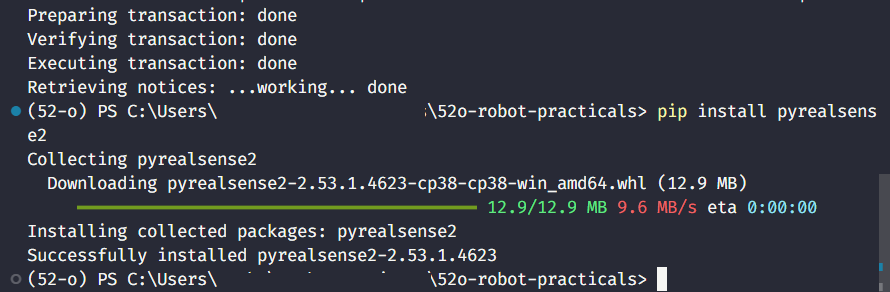
\includegraphics[height=2in]{image/5a_vision.png}
\end{center}

\paragraph{5B. Connect Camera to your machine.}
\begin{center}
    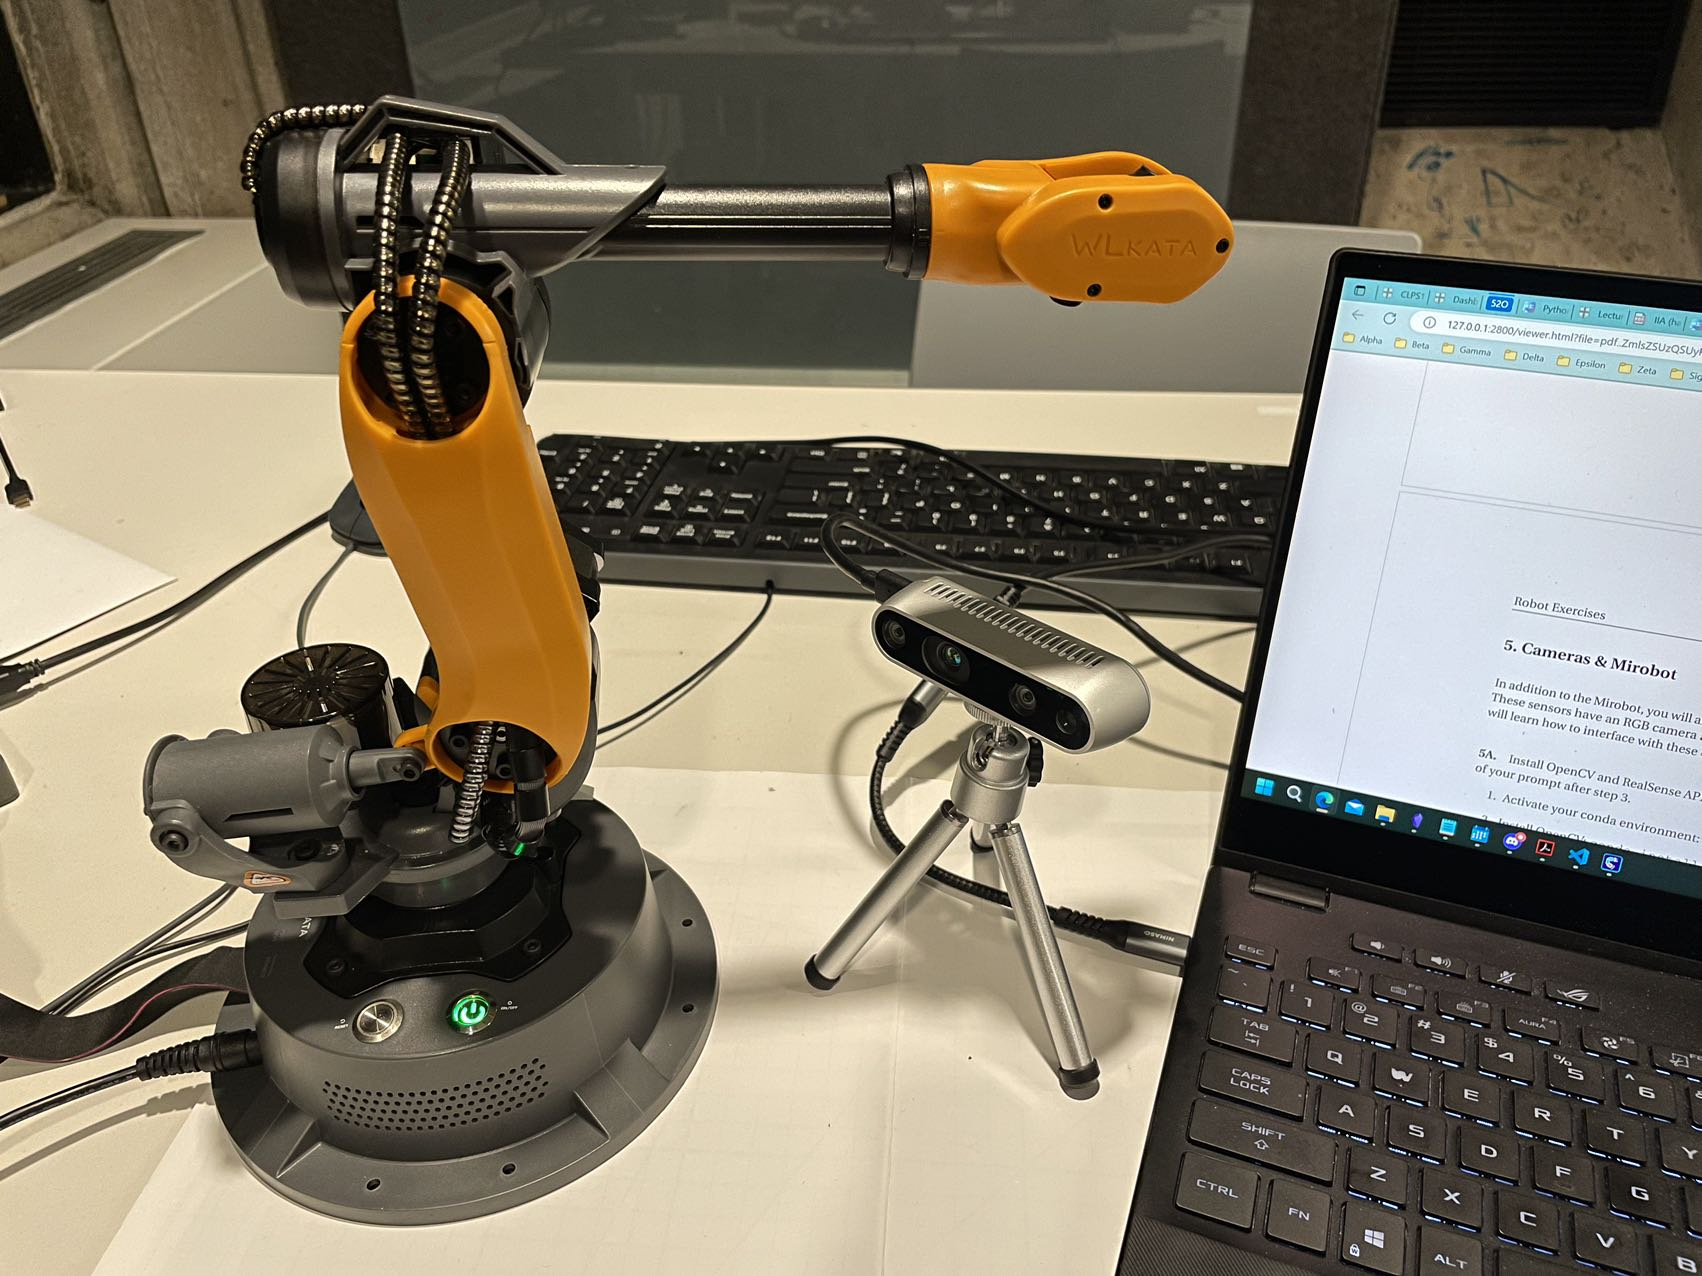
\includegraphics[height=2.5in]{image/5b.jpg}
\end{center}

\newpage
\paragraph{5C. Visualize using OpenCV.}
\begin{center}
    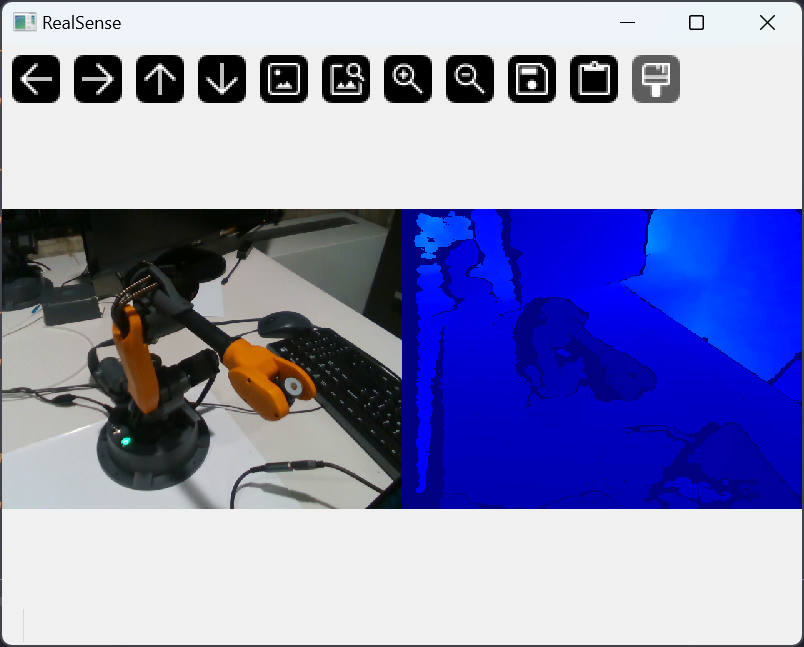
\includegraphics[height=2in]{image/5c.png}
    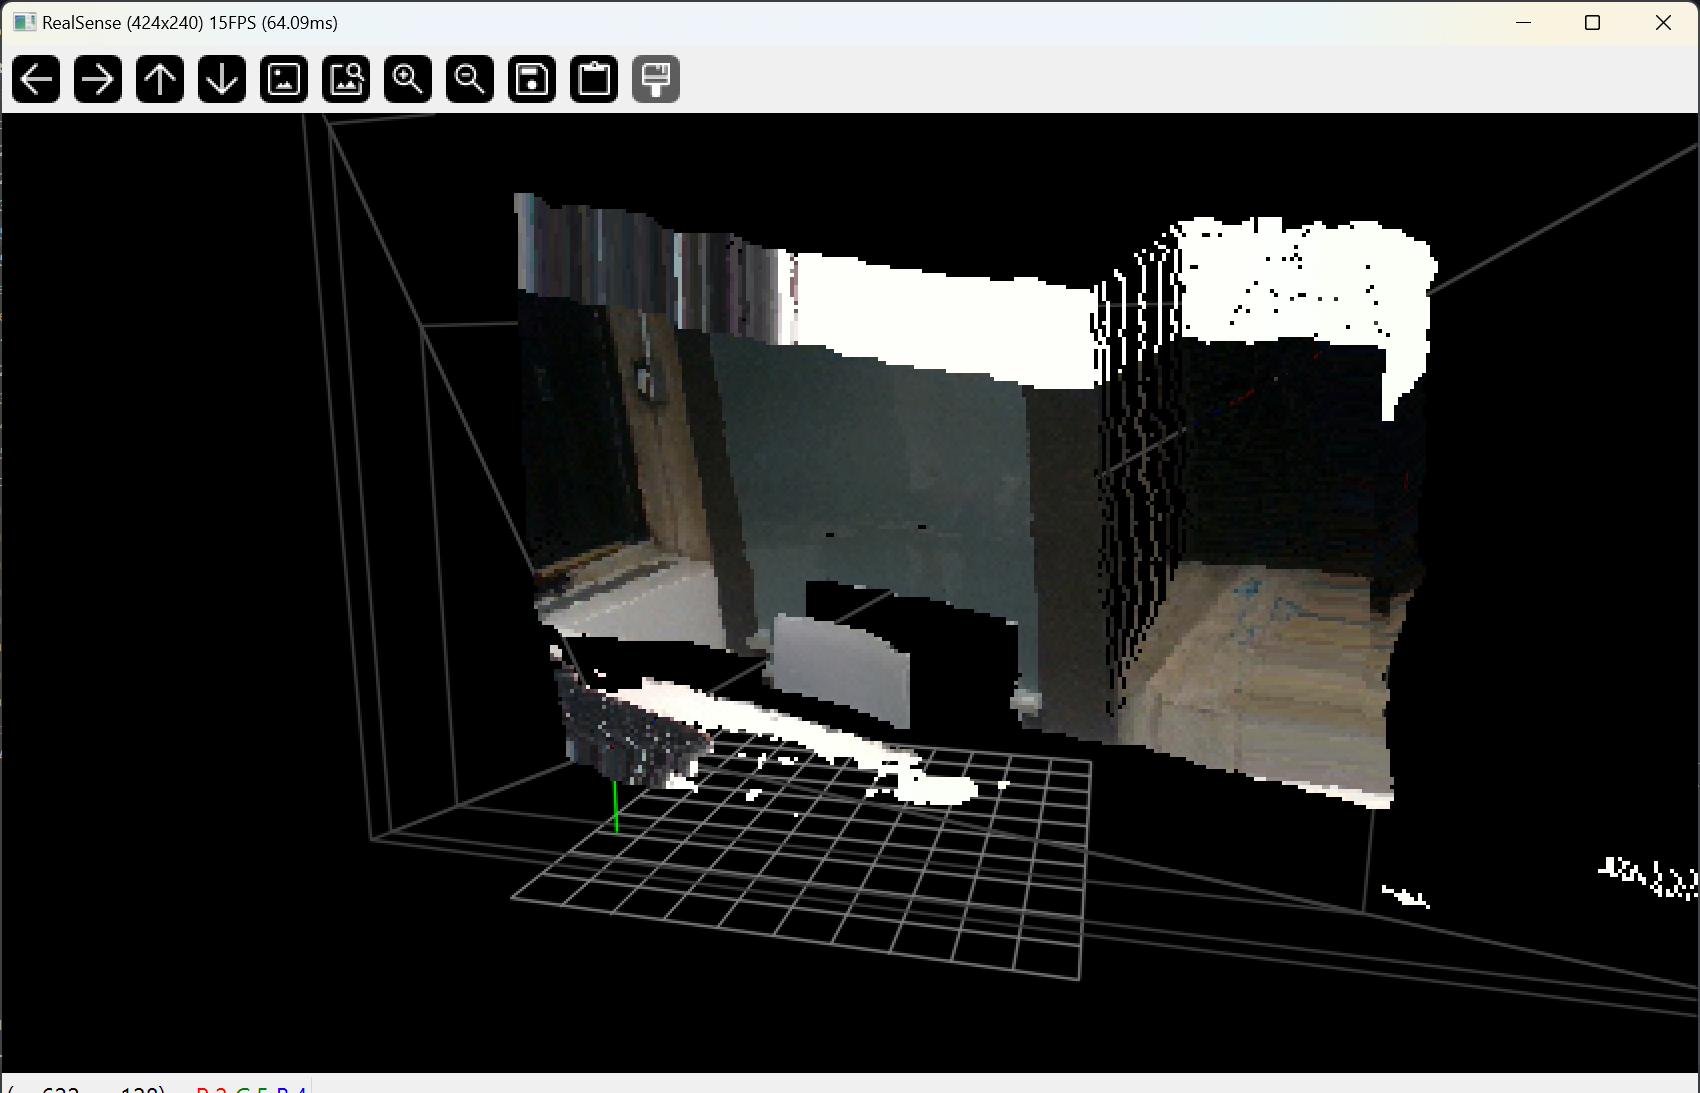
\includegraphics[height=2in]{image/5c_2.png}
\end{center}

\paragraph{5D. Camera Calibration.}
%


The code goes into the appendix pages as it's too long. The script collects images if ran with arguments, and calibrates the camera after that. The screenshot below demonstrates the script running.

\begin{center}
    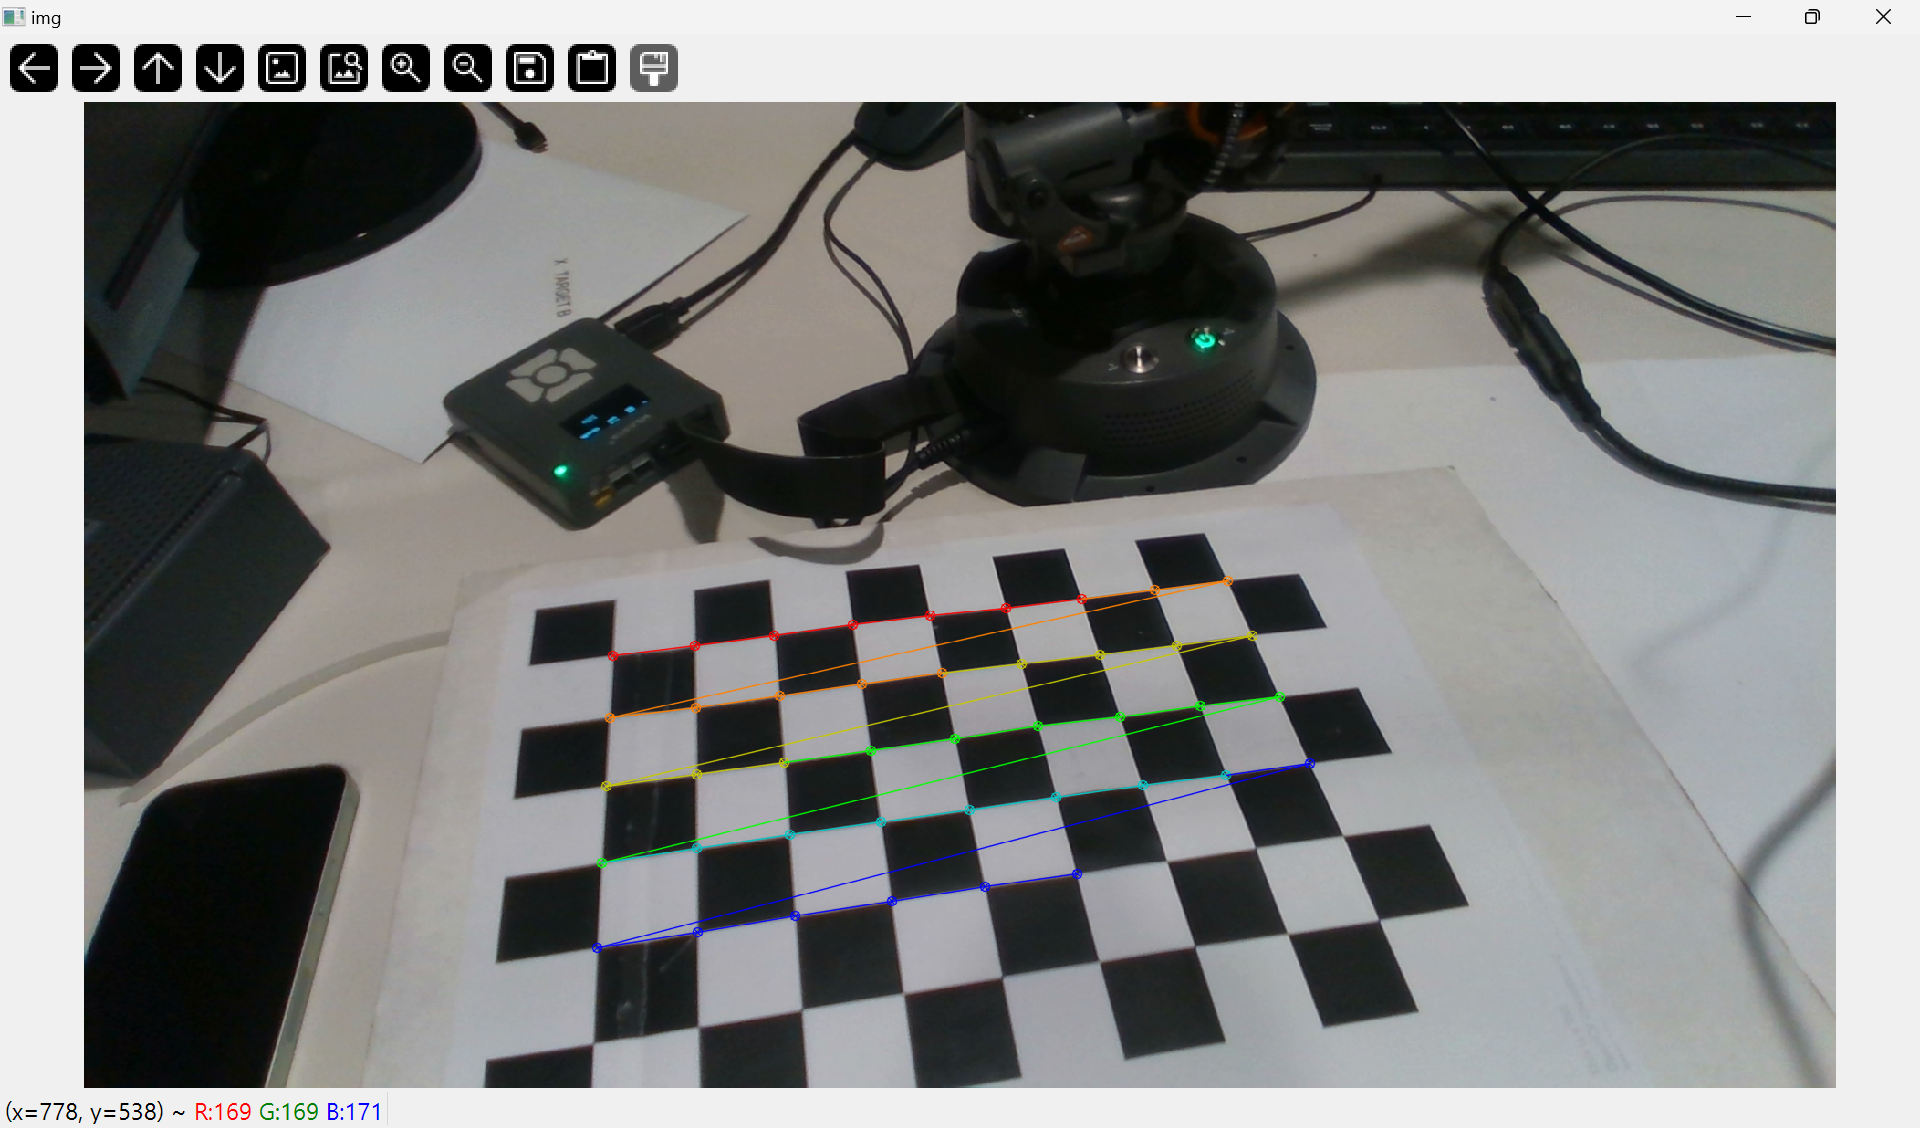
\includegraphics[height=2in]{image/5d_calibration.png}
\end{center}


Please also report the matrix stored in the \texttt{cameraMatrix} return variable of the \texttt{calibrateCamera} function.

The matrix is 
$\begin{bmatrix}
    5.72279816e+01 & 0.00000000e+00 & 5.50917957e+01 \\
    0.00000000e+00 & 6.52853241e+01 & 1.02406546e+03 \\
    0.00000000e+00 & 0.00000000e+00 & 1.00000000e+00 \\
\end{bmatrix}$

\newpage
\paragraph{Additional Space.}
Please do not exceed this page for this question.
\begin{minted}[fontsize=\footnotesize]{python}
import pyrealsense2 as rs
import numpy as np
import cv2
import time
import sys
import glob


    
# termination criteria
criteria = (cv2.TERM_CRITERIA_EPS + cv2.TERM_CRITERIA_MAX_ITER, 30, 0.001)
# prepare object points, like (0,0,0), (1,0,0), (2,0,0) ....,(6,5,0)
objp = np.zeros((6*9,3), np.float32)
objp[:,:2] = np.mgrid[0:9,0:6].T.reshape(-1,2)
# Arrays to store object points and image points from all the images.
objpoints = [] # 3d point in real world space
imgpoints = [] # 2d points in image plane.

if len(sys.argv) > 1:
    # Configure depth and color streams
    pipeline = rs.pipeline()
    config = rs.config()

    # Get device product line for setting a supporting resolution
    pipeline_wrapper = rs.pipeline_wrapper(pipeline)
    pipeline_profile = config.resolve(pipeline_wrapper)
    device = pipeline_profile.get_device()
    device_product_line = str(device.get_info(rs.camera_info.product_line))

    found_rgb = False
    for s in device.sensors:
        if s.get_info(rs.camera_info.name) == 'RGB Camera':
            found_rgb = True
            break
    if not found_rgb:
        print("The demo requires Depth camera with Color sensor")
        exit(0)

    config.enable_stream(rs.stream.depth, 640, 480, rs.format.z16, 30)

    if device_product_line == 'L500':
        config.enable_stream(rs.stream.color, 960, 540, rs.format.bgr8, 30)
    else:
        config.enable_stream(rs.stream.color, 640, 480, rs.format.bgr8, 30)
        
    # Configure depth and color streams
    pipeline = rs.pipeline()
    config = rs.config()

    pipeline_wrapper = rs.pipeline_wrapper(pipeline)
    pipeline_profile = config.resolve(pipeline_wrapper)
    device = pipeline_profile.get_device()

    found_rgb = False
    for s in device.sensors:
        if s.get_info(rs.camera_info.name) == 'RGB Camera':
            found_rgb = True
            break
    if not found_rgb:
        print("The demo requires Depth camera with Color sensor")
        exit(0)

    config.enable_stream(rs.stream.depth, rs.format.z16, 30)
    config.enable_stream(rs.stream.color, rs.format.bgr8, 30)

    # Start streaming
    pipeline.start(config)
    
    # Get images
    k = 1
    while k <= 10:
        frames = pipeline.wait_for_frames()
        color_frame = np.asanyarray(frames.get_color_frame().get_data())
        cv2.imwrite(f'./calibration/out{k}.png', color_frame)
        time.sleep(2)
        print(f"image {k} captured!")
        k += 1

images = glob.glob('./calibration/*.png')
print('images read!')

for fname in  images:
    img = cv2.imread(fname)
    gray = cv2.cvtColor(img, cv2.COLOR_BGR2GRAY)
    # Find the chess board corners
    ret, corners = cv2.findChessboardCorners(gray, (9, 6), None)
    # If found, add object points, image points (after refining them)
    if ret == True:
        objpoints.append(objp)
        corners2 = cv2.cornerSubPix(gray,corners, (11,11), (-1,-1), criteria)
        imgpoints.append(corners2)
        # Draw and display the corners
        cv2.drawChessboardCorners(img, (7,6), corners2, ret)
        cv2.imshow('img', img)
        cv2.waitKey(500)

ret, mtx, dist, rvecs, tvecs = cv2.calibrateCamera(objpoints, imgpoints, gray.shape[::-1], None, None)

img = cv2.imread('./calibration/out1.png')
h,  w = img.shape[:2]
newcameramtx, roi = cv2.getOptimalNewCameraMatrix(mtx, dist, (w,h), 1, (w,h))
print(newcameramtx)

# undistort
dst = cv2.undistort(img, mtx, dist, None, newcameramtx)
# crop the image
x, y, w, h = roi
dst = dst[y:y+h, x:x+w]
cv2.imwrite('calibresult.png', dst)

cv2.destroyAllWindows()
\end{minted}
%%%%%% YOU ANSWER ENDS HERE
